\documentclass[]{article}
\usepackage{lmodern}
\usepackage{amssymb,amsmath}
\usepackage{ifxetex,ifluatex}
\usepackage{fixltx2e} % provides \textsubscript
\ifnum 0\ifxetex 1\fi\ifluatex 1\fi=0 % if pdftex
  \usepackage[T1]{fontenc}
  \usepackage[utf8]{inputenc}
\else % if luatex or xelatex
  \ifxetex
    \usepackage{mathspec}
  \else
    \usepackage{fontspec}
  \fi
  \defaultfontfeatures{Ligatures=TeX,Scale=MatchLowercase}
\fi
% use upquote if available, for straight quotes in verbatim environments
\IfFileExists{upquote.sty}{\usepackage{upquote}}{}
% use microtype if available
\IfFileExists{microtype.sty}{%
\usepackage{microtype}
\UseMicrotypeSet[protrusion]{basicmath} % disable protrusion for tt fonts
}{}
\usepackage[margin=1in]{geometry}
\usepackage{hyperref}
\hypersetup{unicode=true,
            pdftitle={R Study Group - Getting Started with R},
            pdfauthor={William Ou},
            pdfborder={0 0 0},
            breaklinks=true}
\urlstyle{same}  % don't use monospace font for urls
\usepackage{color}
\usepackage{fancyvrb}
\newcommand{\VerbBar}{|}
\newcommand{\VERB}{\Verb[commandchars=\\\{\}]}
\DefineVerbatimEnvironment{Highlighting}{Verbatim}{commandchars=\\\{\}}
% Add ',fontsize=\small' for more characters per line
\usepackage{framed}
\definecolor{shadecolor}{RGB}{248,248,248}
\newenvironment{Shaded}{\begin{snugshade}}{\end{snugshade}}
\newcommand{\KeywordTok}[1]{\textcolor[rgb]{0.13,0.29,0.53}{\textbf{{#1}}}}
\newcommand{\DataTypeTok}[1]{\textcolor[rgb]{0.13,0.29,0.53}{{#1}}}
\newcommand{\DecValTok}[1]{\textcolor[rgb]{0.00,0.00,0.81}{{#1}}}
\newcommand{\BaseNTok}[1]{\textcolor[rgb]{0.00,0.00,0.81}{{#1}}}
\newcommand{\FloatTok}[1]{\textcolor[rgb]{0.00,0.00,0.81}{{#1}}}
\newcommand{\ConstantTok}[1]{\textcolor[rgb]{0.00,0.00,0.00}{{#1}}}
\newcommand{\CharTok}[1]{\textcolor[rgb]{0.31,0.60,0.02}{{#1}}}
\newcommand{\SpecialCharTok}[1]{\textcolor[rgb]{0.00,0.00,0.00}{{#1}}}
\newcommand{\StringTok}[1]{\textcolor[rgb]{0.31,0.60,0.02}{{#1}}}
\newcommand{\VerbatimStringTok}[1]{\textcolor[rgb]{0.31,0.60,0.02}{{#1}}}
\newcommand{\SpecialStringTok}[1]{\textcolor[rgb]{0.31,0.60,0.02}{{#1}}}
\newcommand{\ImportTok}[1]{{#1}}
\newcommand{\CommentTok}[1]{\textcolor[rgb]{0.56,0.35,0.01}{\textit{{#1}}}}
\newcommand{\DocumentationTok}[1]{\textcolor[rgb]{0.56,0.35,0.01}{\textbf{\textit{{#1}}}}}
\newcommand{\AnnotationTok}[1]{\textcolor[rgb]{0.56,0.35,0.01}{\textbf{\textit{{#1}}}}}
\newcommand{\CommentVarTok}[1]{\textcolor[rgb]{0.56,0.35,0.01}{\textbf{\textit{{#1}}}}}
\newcommand{\OtherTok}[1]{\textcolor[rgb]{0.56,0.35,0.01}{{#1}}}
\newcommand{\FunctionTok}[1]{\textcolor[rgb]{0.00,0.00,0.00}{{#1}}}
\newcommand{\VariableTok}[1]{\textcolor[rgb]{0.00,0.00,0.00}{{#1}}}
\newcommand{\ControlFlowTok}[1]{\textcolor[rgb]{0.13,0.29,0.53}{\textbf{{#1}}}}
\newcommand{\OperatorTok}[1]{\textcolor[rgb]{0.81,0.36,0.00}{\textbf{{#1}}}}
\newcommand{\BuiltInTok}[1]{{#1}}
\newcommand{\ExtensionTok}[1]{{#1}}
\newcommand{\PreprocessorTok}[1]{\textcolor[rgb]{0.56,0.35,0.01}{\textit{{#1}}}}
\newcommand{\AttributeTok}[1]{\textcolor[rgb]{0.77,0.63,0.00}{{#1}}}
\newcommand{\RegionMarkerTok}[1]{{#1}}
\newcommand{\InformationTok}[1]{\textcolor[rgb]{0.56,0.35,0.01}{\textbf{\textit{{#1}}}}}
\newcommand{\WarningTok}[1]{\textcolor[rgb]{0.56,0.35,0.01}{\textbf{\textit{{#1}}}}}
\newcommand{\AlertTok}[1]{\textcolor[rgb]{0.94,0.16,0.16}{{#1}}}
\newcommand{\ErrorTok}[1]{\textcolor[rgb]{0.64,0.00,0.00}{\textbf{{#1}}}}
\newcommand{\NormalTok}[1]{{#1}}
\usepackage{graphicx,grffile}
\makeatletter
\def\maxwidth{\ifdim\Gin@nat@width>\linewidth\linewidth\else\Gin@nat@width\fi}
\def\maxheight{\ifdim\Gin@nat@height>\textheight\textheight\else\Gin@nat@height\fi}
\makeatother
% Scale images if necessary, so that they will not overflow the page
% margins by default, and it is still possible to overwrite the defaults
% using explicit options in \includegraphics[width, height, ...]{}
\setkeys{Gin}{width=\maxwidth,height=\maxheight,keepaspectratio}
\IfFileExists{parskip.sty}{%
\usepackage{parskip}
}{% else
\setlength{\parindent}{0pt}
\setlength{\parskip}{6pt plus 2pt minus 1pt}
}
\setlength{\emergencystretch}{3em}  % prevent overfull lines
\providecommand{\tightlist}{%
  \setlength{\itemsep}{0pt}\setlength{\parskip}{0pt}}
\setcounter{secnumdepth}{0}
% Redefines (sub)paragraphs to behave more like sections
\ifx\paragraph\undefined\else
\let\oldparagraph\paragraph
\renewcommand{\paragraph}[1]{\oldparagraph{#1}\mbox{}}
\fi
\ifx\subparagraph\undefined\else
\let\oldsubparagraph\subparagraph
\renewcommand{\subparagraph}[1]{\oldsubparagraph{#1}\mbox{}}
\fi

%%% Use protect on footnotes to avoid problems with footnotes in titles
\let\rmarkdownfootnote\footnote%
\def\footnote{\protect\rmarkdownfootnote}

%%% Change title format to be more compact
\usepackage{titling}

% Create subtitle command for use in maketitle
\providecommand{\subtitle}[1]{
  \posttitle{
    \begin{center}\large#1\end{center}
    }
}

\setlength{\droptitle}{-2em}

  \title{R Study Group - Getting Started with R}
    \pretitle{\vspace{\droptitle}\centering\huge}
  \posttitle{\par}
    \author{William Ou}
    \preauthor{\centering\large\emph}
  \postauthor{\par}
      \predate{\centering\large\emph}
  \postdate{\par}
    \date{9/24/2019}


\begin{document}
\maketitle

\subsection{Why use R?}\label{why-use-r}

\begin{enumerate}
\def\labelenumi{\arabic{enumi}.}
\tightlist
\item
  Clean and fast way of doing repetitive things
\item
  Reproducible (anyone with your script can do exactly what you did)
\item
  Easy calculations
\item
  Data wrangling: cleaning and organizing data
\item
  Data visualization
\item
  Tons of libraries for you to use - libraries are essentially functions
  that people have written already that you can use
\item
  A friendly community where everyone helps everyone!
\end{enumerate}

Any thing else?

\subsection{What is R Studio?}\label{what-is-r-studio}

\begin{itemize}
\tightlist
\item
  an open-source Integrated Development Environment (IDE) for R
\item
  helps you keep track of things
\end{itemize}

\begin{enumerate}
\def\labelenumi{\arabic{enumi}.}
\tightlist
\item
  Code Editor - Basically your note pad or sketch pad for code
\item
  R Console - This is what R itself actually is -- where your executed
  code goes to and where the output of those executed code shows, too
\item
  Workspace \& History- Keeps track of all the variables you have
  assigned, data you have loaded, and code that you executed
\item
  Plots and files - The graphical device of your plots and shows where
  your files are (not too useful IMO)
\end{enumerate}

\paragraph{R Studio interface}\label{r-studio-interface}

\begin{center}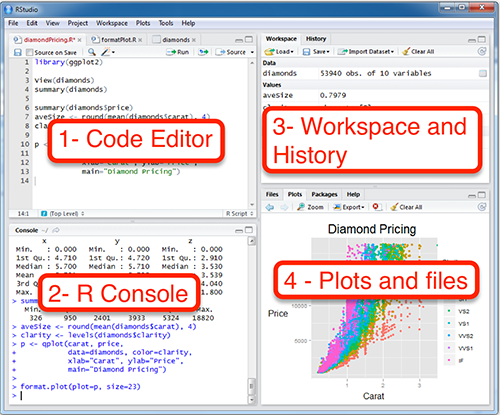
\includegraphics[width=400px]{/Users/jiaangou/Desktop/rstudio-interface} \end{center}

\subsection{R syntax and defintions}\label{r-syntax-and-defintions}

\begin{itemize}
\tightlist
\item
  ``\textless{}-'' is used to assign a value or object to a variable
\end{itemize}

\begin{Shaded}
\begin{Highlighting}[]
\NormalTok{a <-}\StringTok{ }\DecValTok{3} \CommentTok{# The value 3 is assigned to the variable a}
\NormalTok{a}
\end{Highlighting}
\end{Shaded}

\begin{verbatim}
## [1] 3
\end{verbatim}

\begin{Shaded}
\begin{Highlighting}[]
\NormalTok{a +}\StringTok{ }\DecValTok{1}
\end{Highlighting}
\end{Shaded}

\begin{verbatim}
## [1] 4
\end{verbatim}

\begin{Shaded}
\begin{Highlighting}[]
\NormalTok{A }\CommentTok{#R is case sensitive! }
\end{Highlighting}
\end{Shaded}

\begin{verbatim}
## Error in eval(expr, envir, enclos): object 'A' not found
\end{verbatim}

\subsection{1. Operators}\label{operators}

\paragraph{1a. Arithmetic: +, -, /, *}\label{a.-arithmetic--}

\begin{Shaded}
\begin{Highlighting}[]
\DecValTok{1+1}
\end{Highlighting}
\end{Shaded}

\begin{verbatim}
## [1] 2
\end{verbatim}

\begin{Shaded}
\begin{Highlighting}[]
\DecValTok{1-5}
\end{Highlighting}
\end{Shaded}

\begin{verbatim}
## [1] -4
\end{verbatim}

\begin{Shaded}
\begin{Highlighting}[]
\DecValTok{1+5}\NormalTok{/}\DecValTok{2} \CommentTok{#Order of operations still holds!}
\end{Highlighting}
\end{Shaded}

\begin{verbatim}
## [1] 3.5
\end{verbatim}

\begin{Shaded}
\begin{Highlighting}[]
\DecValTok{2}\NormalTok{*}\DecValTok{4-2}
\end{Highlighting}
\end{Shaded}

\begin{verbatim}
## [1] 6
\end{verbatim}

\paragraph{1b. Logical or Boolean:
\textgreater{},\textless{},\textless{}=,\textgreater{}=,==,
!=}\label{b.-logical-or-boolean}

\begin{Shaded}
\begin{Highlighting}[]
\DecValTok{1}\NormalTok{>}\DecValTok{3} \CommentTok{#greater than}
\end{Highlighting}
\end{Shaded}

\begin{verbatim}
## [1] FALSE
\end{verbatim}

\begin{Shaded}
\begin{Highlighting}[]
\DecValTok{1}\NormalTok{>=}\FloatTok{0.1} \CommentTok{#greater than or equal to}
\end{Highlighting}
\end{Shaded}

\begin{verbatim}
## [1] TRUE
\end{verbatim}

\begin{Shaded}
\begin{Highlighting}[]
\DecValTok{1}\NormalTok{<=}\DecValTok{4} \CommentTok{#less than or equal to}
\end{Highlighting}
\end{Shaded}

\begin{verbatim}
## [1] TRUE
\end{verbatim}

\begin{Shaded}
\begin{Highlighting}[]
\DecValTok{112}\NormalTok{==}\DecValTok{2} \CommentTok{#equal to}
\end{Highlighting}
\end{Shaded}

\begin{verbatim}
## [1] FALSE
\end{verbatim}

\begin{Shaded}
\begin{Highlighting}[]
\DecValTok{15}\NormalTok{!=}\DecValTok{2} \CommentTok{#not equal to}
\end{Highlighting}
\end{Shaded}

\begin{verbatim}
## [1] TRUE
\end{verbatim}

\subsubsection{\texorpdfstring{2. Class (or the ``type'' of
object)}{2. Class (or the type of object)}}\label{class-or-the-type-of-object}

\begin{itemize}
\tightlist
\item
  This is usually the cause of all problems!
\item
  Most functions can only accept a certain ``class'' of object as input.
  When it is not, you will get an error message
\item
  Whenever you get an error message, check if your objects are the right
  class!
\end{itemize}

\paragraph{2a. Numeric - outputs of arithmetic expressions are
numeric}\label{a.-numeric---outputs-of-arithmetic-expressions-are-numeric}

\begin{Shaded}
\begin{Highlighting}[]
\KeywordTok{class}\NormalTok{(}\DecValTok{5+1}\NormalTok{)}
\end{Highlighting}
\end{Shaded}

\begin{verbatim}
## [1] "numeric"
\end{verbatim}

\paragraph{2b. Logical - output of logical/boolean
expressions}\label{b.-logical---output-of-logicalboolean-expressions}

\begin{itemize}
\tightlist
\item
  These are essentially binary outputs (ie. TRUE = 1 and FALSE = 0)
\item
  In R, you can apply arithmetic operators to TRUE and FALSE
\end{itemize}

\begin{Shaded}
\begin{Highlighting}[]
\KeywordTok{class}\NormalTok{(}\DecValTok{5}\NormalTok{>}\DecValTok{2}\NormalTok{)}
\end{Highlighting}
\end{Shaded}

\begin{verbatim}
## [1] "logical"
\end{verbatim}

\begin{Shaded}
\begin{Highlighting}[]
\NormalTok{(}\DecValTok{5}\NormalTok{>}\DecValTok{2}\NormalTok{)+(}\DecValTok{1}\NormalTok{==}\DecValTok{1}\NormalTok{)}
\end{Highlighting}
\end{Shaded}

\begin{verbatim}
## [1] 2
\end{verbatim}

\begin{Shaded}
\begin{Highlighting}[]
\KeywordTok{class}\NormalTok{((}\DecValTok{5}\NormalTok{>}\DecValTok{2}\NormalTok{)+(}\DecValTok{1}\NormalTok{==}\DecValTok{1}\NormalTok{)) }\CommentTok{#}
\end{Highlighting}
\end{Shaded}

\begin{verbatim}
## [1] "integer"
\end{verbatim}

\begin{itemize}
\tightlist
\item
  this one is an integer, which generally works the same as numeric. The
  main difference has something to do with how the memory is stored in
  the machine\ldots{} TLDR not important but watch out
\end{itemize}

\paragraph{\texorpdfstring{2c. Character or
``string''}{2c. Character or string}}\label{c.-character-or-string}

\begin{itemize}
\tightlist
\item
  non-numerical ``values'' like words (but numerical values can be
  stored as charcaters too!)
\item
  these values are specified with quotation marks ``'' or ''
\item
  letters or words without ``'' marks are read by R as variables
\item
  \textbf{\emph{NOTE: characters are sometimes automatically converted
  to another class known as ``factors'', like categorical variables in
  an ANOVA }}
\end{itemize}

\begin{Shaded}
\begin{Highlighting}[]
\NormalTok{sentence <-}\StringTok{ "Hello, mortals."}
\KeywordTok{print}\NormalTok{(sentence)}
\end{Highlighting}
\end{Shaded}

\begin{verbatim}
## [1] "Hello, mortals."
\end{verbatim}

\begin{Shaded}
\begin{Highlighting}[]
\KeywordTok{class}\NormalTok{(sentence)}
\end{Highlighting}
\end{Shaded}

\begin{verbatim}
## [1] "character"
\end{verbatim}

\begin{Shaded}
\begin{Highlighting}[]
\KeywordTok{print}\NormalTok{(}\StringTok{'sentence'}\NormalTok{) }\CommentTok{#by adding '', the letters in senetence is a charcater object }
\end{Highlighting}
\end{Shaded}

\begin{verbatim}
## [1] "sentence"
\end{verbatim}

\begin{Shaded}
\begin{Highlighting}[]
\CommentTok{#and not the variable that I have previously assigned}
\KeywordTok{class}\NormalTok{(}\StringTok{'5193'}\NormalTok{) }
\end{Highlighting}
\end{Shaded}

\begin{verbatim}
## [1] "character"
\end{verbatim}

\begin{Shaded}
\begin{Highlighting}[]
\KeywordTok{class}\NormalTok{(}\DecValTok{5193}\NormalTok{)}
\end{Highlighting}
\end{Shaded}

\begin{verbatim}
## [1] "numeric"
\end{verbatim}

\begin{Shaded}
\begin{Highlighting}[]
\StringTok{'5123'}\NormalTok{+}\DecValTok{3} \CommentTok{#common mistake/error !!}
\end{Highlighting}
\end{Shaded}

\begin{verbatim}
## Error in "5123" + 3: non-numeric argument to binary operator
\end{verbatim}

\paragraph{2d. Factors}\label{d.-factors}

\begin{itemize}
\tightlist
\item
  factors are almost identical to characters, in fact, they are
  interchangeable sometimes
\item
  are more commonly used in terms of data analysis
\item
  differ from characters in that they have ``levels'', or unique entries
  in the vector of factor elements
\end{itemize}

\begin{Shaded}
\begin{Highlighting}[]
\NormalTok{char <-}\StringTok{ }\KeywordTok{c}\NormalTok{(}\StringTok{'a'}\NormalTok{,}\StringTok{'a'}\NormalTok{,}\StringTok{'a'}\NormalTok{,}\StringTok{'b'}\NormalTok{,}\StringTok{'d'}\NormalTok{,}\StringTok{'d'}\NormalTok{,}\StringTok{'d'}\NormalTok{) }\CommentTok{#a character vector}
\NormalTok{char}
\end{Highlighting}
\end{Shaded}

\begin{verbatim}
## [1] "a" "a" "a" "b" "d" "d" "d"
\end{verbatim}

\begin{Shaded}
\begin{Highlighting}[]
\KeywordTok{factor}\NormalTok{(char)}
\end{Highlighting}
\end{Shaded}

\begin{verbatim}
## [1] a a a b d d d
## Levels: a b d
\end{verbatim}

\begin{itemize}
\tightlist
\item
  By default, factor levels will be sorted alphabetically (or
  numerically if the factors are numbers)
\item
  This can be changed by including an additional argument in the
  \textbf{\emph{factor()}} function:
\end{itemize}

\begin{Shaded}
\begin{Highlighting}[]
\NormalTok{new_fact <-}\StringTok{ }\KeywordTok{factor}\NormalTok{(char)}
\KeywordTok{factor}\NormalTok{(new_fact,}\DataTypeTok{levels=}\KeywordTok{c}\NormalTok{(}\StringTok{'d'}\NormalTok{,}\StringTok{'a'}\NormalTok{,}\StringTok{'b'}\NormalTok{))}
\end{Highlighting}
\end{Shaded}

\begin{verbatim}
## [1] a a a b d d d
## Levels: d a b
\end{verbatim}

\paragraph{Converting between classes}\label{converting-between-classes}

\begin{itemize}
\tightlist
\item
  you can use built-in function in R to convert between classes
\item
  it usually looks something like as.\emph{class to convert to} ()
\end{itemize}

\begin{Shaded}
\begin{Highlighting}[]
\NormalTok{v <-}\StringTok{ }\KeywordTok{c}\NormalTok{(}\DecValTok{1}\NormalTok{,}\DecValTok{2}\NormalTok{,}\DecValTok{4}\NormalTok{,}\DecValTok{2}\NormalTok{)}
\KeywordTok{as.factor}\NormalTok{(v) }\CommentTok{#to factor}
\end{Highlighting}
\end{Shaded}

\begin{verbatim}
## [1] 1 2 4 2
## Levels: 1 2 4
\end{verbatim}

\begin{Shaded}
\begin{Highlighting}[]
\KeywordTok{as.character}\NormalTok{(v)}
\end{Highlighting}
\end{Shaded}

\begin{verbatim}
## [1] "1" "2" "4" "2"
\end{verbatim}

\begin{Shaded}
\begin{Highlighting}[]
\KeywordTok{as.integer}\NormalTok{(v)}
\end{Highlighting}
\end{Shaded}

\begin{verbatim}
## [1] 1 2 4 2
\end{verbatim}

\subsection{Data structures}\label{data-structures}

\begin{center}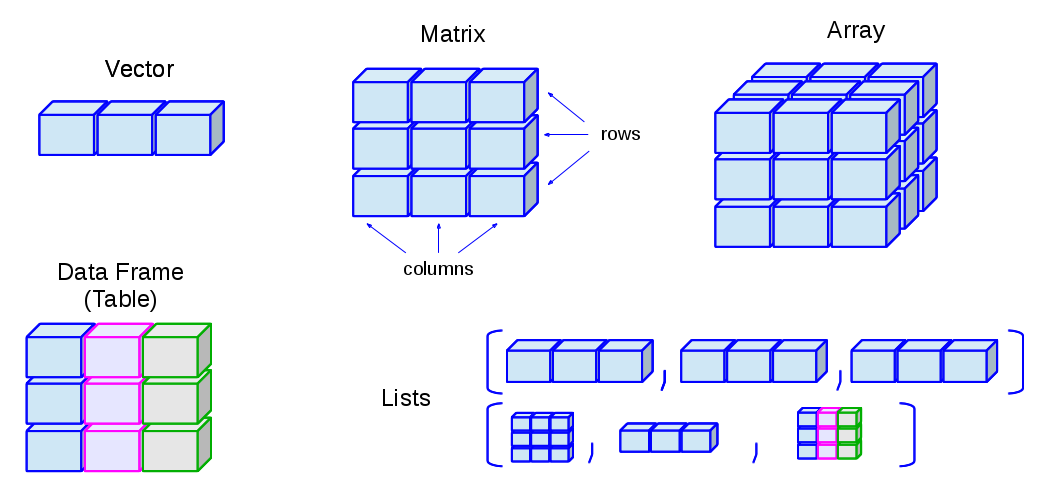
\includegraphics[width=300px]{/Users/jiaangou/Desktop/RDataStructures} \end{center}

\paragraph{1. Vectors}\label{vectors}

\begin{itemize}
\tightlist
\item
  A series of n-elements in which all elements are of the same class
\item
  Key here is that everything is of the same class!
\item
  Becuase all elements are of the same class, the class() function
  returns the class of the objects and not a ``vector'' class (ie. there
  is no ``vector'' class)
\item
  to create a vector, you can use c()
\end{itemize}

Indexing: \textbf{\emph{vec{[}i{]}}} (ie. the \emph{ith} element of
vector \emph{vec})

\begin{Shaded}
\begin{Highlighting}[]
\KeywordTok{c}\NormalTok{(}\DecValTok{1}\NormalTok{,}\DecValTok{2}\NormalTok{,}\DecValTok{5}\NormalTok{,}\DecValTok{2}\NormalTok{) }\CommentTok{# vector of integers/numerical values}
\end{Highlighting}
\end{Shaded}

\begin{verbatim}
## [1] 1 2 5 2
\end{verbatim}

\begin{Shaded}
\begin{Highlighting}[]
\KeywordTok{class}\NormalTok{(}\KeywordTok{c}\NormalTok{(}\DecValTok{1}\NormalTok{,}\DecValTok{2}\NormalTok{,}\DecValTok{5}\NormalTok{,}\DecValTok{2}\NormalTok{))}
\end{Highlighting}
\end{Shaded}

\begin{verbatim}
## [1] "numeric"
\end{verbatim}

\begin{Shaded}
\begin{Highlighting}[]
\KeywordTok{class}\NormalTok{(}\KeywordTok{c}\NormalTok{(}\DecValTok{2}\NormalTok{,}\DecValTok{2}\NormalTok{,}\DecValTok{4}\NormalTok{,}\StringTok{'bb'}\NormalTok{)) }\CommentTok{#numerical values are forced as characters}
\end{Highlighting}
\end{Shaded}

\begin{verbatim}
## [1] "character"
\end{verbatim}

\begin{Shaded}
\begin{Highlighting}[]
\KeywordTok{length}\NormalTok{(}\KeywordTok{c}\NormalTok{(}\DecValTok{1}\NormalTok{,}\DecValTok{2}\NormalTok{,}\DecValTok{4}\NormalTok{,}\DecValTok{5}\NormalTok{,}\DecValTok{14}\NormalTok{)) }\CommentTok{#length() is a function that tells you the number of elements of your object}
\end{Highlighting}
\end{Shaded}

\begin{verbatim}
## [1] 5
\end{verbatim}

\paragraph{BONUS!! A cool thing about vectors: It makes things
faster!}\label{bonus-a-cool-thing-about-vectors-it-makes-things-faster}

\begin{itemize}
\tightlist
\item
  You might hear people say that a solution or algorithm is
  ``vectorized'', and this is what they are talking about.
\end{itemize}

Say we have a numeric vector, \emph{vec}:

\begin{Shaded}
\begin{Highlighting}[]
\NormalTok{vec <-}\StringTok{ }\KeywordTok{c}\NormalTok{(}\DecValTok{1}\NormalTok{,}\DecValTok{2}\NormalTok{,}\DecValTok{4}\NormalTok{,}\DecValTok{2}\NormalTok{,}\DecValTok{5}\NormalTok{)}
\NormalTok{vec}
\end{Highlighting}
\end{Shaded}

\begin{verbatim}
## [1] 1 2 4 2 5
\end{verbatim}

Imagine we want to add 1 to all of the elements of \emph{vec}. One way
to do it is to iterate through each of the vector elements and add 1 to
each iteration, like so:

\begin{Shaded}
\begin{Highlighting}[]
\CommentTok{# for loop}
\KeywordTok{system.time}\NormalTok{(for (i in }\DecValTok{1}\NormalTok{:}\KeywordTok{length}\NormalTok{(vec))\{}
  \NormalTok{vec[i] <-}\StringTok{ }\NormalTok{vec[i]+}\DecValTok{1}
  \NormalTok{\})}
\end{Highlighting}
\end{Shaded}

\begin{verbatim}
##    user  system elapsed 
##   0.016   0.001   0.018
\end{verbatim}

\begin{Shaded}
\begin{Highlighting}[]
\NormalTok{vec}
\end{Highlighting}
\end{Shaded}

\begin{verbatim}
## [1] 2 3 5 3 6
\end{verbatim}

\textbf{OR} Option 2, we could just simply +1 to the whole vector

\begin{Shaded}
\begin{Highlighting}[]
\KeywordTok{system.time}\NormalTok{(vec <-}\StringTok{ }\NormalTok{vec}\DecValTok{+1}\NormalTok{)}
\end{Highlighting}
\end{Shaded}

\begin{verbatim}
##    user  system elapsed 
##       0       0       0
\end{verbatim}

\begin{Shaded}
\begin{Highlighting}[]
\NormalTok{vec}
\end{Highlighting}
\end{Shaded}

\begin{verbatim}
## [1] 3 4 6 4 7
\end{verbatim}

Option 2 is so fast that the decimals were not enough to show the time!
Although Option 1 was pretty fast too (0.002s), these kind of
computations will become extremely long to compute when you have a LARGE
data set (eg. 10000+). Moreover, Option 2 is also just a more elegant
piece of code!

\paragraph{2. Data frames}\label{data-frames}

\begin{itemize}
\tightlist
\item
  This is probably what you will work with the most, so get familiar
  with it!
\item
  The best way to describe a data frame is that it is a list of vectors,
  in which each column is a vector and the rows are the elements of the
  vector
\item
  Following this description, elements within a column of a dataframe
  should always be of the same class while elements between columns do
  not necessarily have to!
\item
  This brings up another important point: Data should \textbf{ALWAYS} be
  organized in the long format! Ie. Each column should represent a
  single variable and rows should be represent 1 some sample of
  that/those variable/s
\end{itemize}

Indexing: - Data frames are indexed by the notation
\emph{df{[}row,column{]}} (eg. row 1 column 3 of df is df{[}1,3{]}) - \$
notation can be also used to index the columns of data frames

\begin{Shaded}
\begin{Highlighting}[]
\NormalTok{df <-}\StringTok{ }\KeywordTok{data.frame}\NormalTok{(}\DataTypeTok{x=}\KeywordTok{c}\NormalTok{(}\DecValTok{2}\NormalTok{,}\DecValTok{4}\NormalTok{,}\DecValTok{1}\NormalTok{,}\DecValTok{5}\NormalTok{,}\DecValTok{9}\NormalTok{),}\DataTypeTok{y=}\KeywordTok{c}\NormalTok{(}\StringTok{'b'}\NormalTok{,}\StringTok{'b'}\NormalTok{,}\StringTok{'b'}\NormalTok{,}\StringTok{'a'}\NormalTok{,}\StringTok{'a'}\NormalTok{))}
\NormalTok{df}
\end{Highlighting}
\end{Shaded}

\begin{verbatim}
##   x y
## 1 2 b
## 2 4 b
## 3 1 b
## 4 5 a
## 5 9 a
\end{verbatim}

\begin{Shaded}
\begin{Highlighting}[]
\NormalTok{df$x }\CommentTok{#outputs the vector x of data frame df}
\end{Highlighting}
\end{Shaded}

\begin{verbatim}
## [1] 2 4 1 5 9
\end{verbatim}

\begin{Shaded}
\begin{Highlighting}[]
\KeywordTok{class}\NormalTok{(df$x)}
\end{Highlighting}
\end{Shaded}

\begin{verbatim}
## [1] "numeric"
\end{verbatim}

\begin{Shaded}
\begin{Highlighting}[]
\KeywordTok{class}\NormalTok{(df$y)}
\end{Highlighting}
\end{Shaded}

\begin{verbatim}
## [1] "factor"
\end{verbatim}

\begin{Shaded}
\begin{Highlighting}[]
\NormalTok{df[}\DecValTok{2}\NormalTok{,] }\CommentTok{#outputs row 2 of every column; empty column means all columns are selected}
\end{Highlighting}
\end{Shaded}

\begin{verbatim}
##   x y
## 2 4 b
\end{verbatim}

\begin{Shaded}
\begin{Highlighting}[]
\NormalTok{df[,}\DecValTok{1}\NormalTok{] }\CommentTok{#same as df$x but using indices instead of the variable name}
\end{Highlighting}
\end{Shaded}

\begin{verbatim}
## [1] 2 4 1 5 9
\end{verbatim}

\newpage

\textbf{What's wrong with this?}

\begin{center}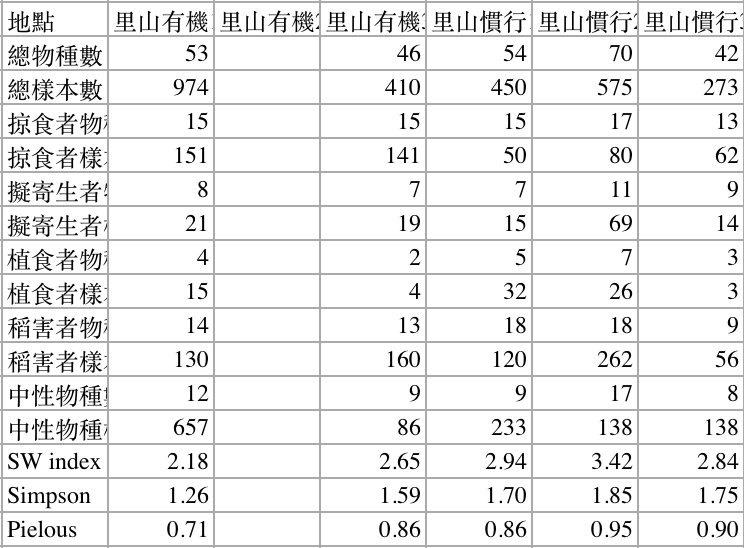
\includegraphics[width=300px]{/Users/jiaangou/Desktop/BadData} \end{center}

\paragraph{3. Matrices}\label{matrices}

\begin{itemize}
\tightlist
\item
  \emph{To be continued}
\end{itemize}

\paragraph{4. Lists}\label{lists}

\begin{itemize}
\tightlist
\item
  \emph{To be continued}
\end{itemize}

\subsubsection{Excercise: Create a new vector from an existing one that
has its elements shifted to the right (1st becomes 2nd and last becomes
the
first)}\label{excercise-create-a-new-vector-from-an-existing-one-that-has-its-elements-shifted-to-the-right-1st-becomes-2nd-and-last-becomes-the-first}

\begin{itemize}
\tightlist
\item
  if the original vector is c(5,3,1,2), return the vector c(2,5,3,1)
\item
  There are multiple ways to do it but the BEST answer is one that is
  generalized and works for any vector
\item
  HINT: try using length() and seq(); use ?seq (or ?length) to see what
  it does
\end{itemize}

\subsubsection{Loading data}\label{loading-data}

\begin{itemize}
\tightlist
\item
  There are numerous ways to load data, usually it depends on the format
  (.csv, .txt, .xlsx etc.) of data you are loading
\item
  As much as possible, don't use excel because of formatting issues
\item
  tab delimited files are the most stable
\item
  you can directly load data by its name if you are working directory is
  in the same as where the file is
\item
  or you can load it by providing the path of the file
\end{itemize}

\begin{Shaded}
\begin{Highlighting}[]
\NormalTok{dat <-}\StringTok{ }\KeywordTok{read.csv}\NormalTok{(}\StringTok{'zooplankton_clean.csv'}\NormalTok{)}

\NormalTok{dat <-}\StringTok{ }\KeywordTok{read.csv}\NormalTok{(}\StringTok{'/Users/jiaangou/Desktop/RStudyGroup/zooplankton_clean.csv'}\NormalTok{)}

\NormalTok{dat <-}\StringTok{ }\KeywordTok{read.csv}\NormalTok{(}\StringTok{"https://www.dropbox.com/s/k3xvoi2vxg9p64k/zooplankton_clean.csv?dl=1"}\NormalTok{)}
\end{Highlighting}
\end{Shaded}

\subsubsection{\texorpdfstring{Data manipulation with \emph{tidyverse}
package}{Data manipulation with tidyverse package}}\label{data-manipulation-with-tidyverse-package}

\begin{itemize}
\tightlist
\item
  \emph{tidyverse} is a series of packages which was created to make
  data science as ``tidy'' as possible
\item
  Useful for quick and clean manipulation and visualization (ggplot) of
  complex data
\item
  It has its own unique syntax, which is often more intuitive than base
  R (IMO)
\item
  \textbf{\emph{Problem}}: Too many different packages and too many
  different functions that sometimes do the similar things. Also a lot
  of error
\item
  Thankfully, there are a lot of cheatsheets and people are helpful
\end{itemize}

\subsubsection{Install and loading
library}\label{install-and-loading-library}

\begin{Shaded}
\begin{Highlighting}[]
\KeywordTok{install.packages}\NormalTok{(}\StringTok{'tidyverse'}\NormalTok{)}
\KeywordTok{library}\NormalTok{(tidyverse)}
\end{Highlighting}
\end{Shaded}

\subsubsection{Practice data set: Zooplankton body sizes across 4
different lakes in
BC}\label{practice-data-set-zooplankton-body-sizes-across-4-different-lakes-in-bc}

Load directly from dropbox:

\begin{Shaded}
\begin{Highlighting}[]
\NormalTok{zooplankton <-}\StringTok{ }\KeywordTok{read.csv}\NormalTok{(}\StringTok{"https://www.dropbox.com/s/500av3zullmiti7/zooplankton.csv?dl=1"}\NormalTok{)}
\end{Highlighting}
\end{Shaded}

\begin{itemize}
\tightlist
\item
  Inspect the data set first. Some helpful functions to help you do so:
  View(), head(), str()
\item
  Make some easy plots: hist(), boxplot(y\textasciitilde{}x)
\item
  If you inspect the genus variable more closely you might find some
  errors
\end{itemize}


\end{document}
